\documentclass{article}

\usepackage{tikz}
\usetikzlibrary{calc,positioning,intersections,arrows,shapes.geometric,shapes.arrows}

\pgfdeclarelayer{background}
\pgfsetlayers{background,main}

\usepackage{gnuplot-lua-tikz}


\begin{document}

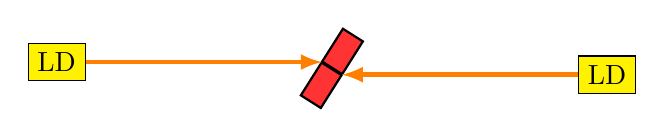
\begin{tikzpicture}
  % laser crystal
  \draw [thick, fill=red!80]
    (0,0) 
    -- ++(-32.3:3mm)
    -- ++(-122.3:10mm)
      coordinate [pos=0.5] (crystal right)
    -- ++(147.7:3mm)
    -- ++(57.7:10mm)
      coordinate [pos=0.5] (crystal left)
    -- cycle
  ;
  % beam path in crystal
  \draw [very thick] (crystal left) -- (crystal right);

  % pump lasers
  \node [left=3 of crystal left, fill=yellow, draw] (LD left) {LD};
  \draw [orange, ultra thick, -latex]
    (LD left)
    -- (crystal left)
  ;
  \node [right=3 of crystal right, fill=yellow, draw] (LD right) {LD};
  \draw [orange, ultra thick, -latex]
    (LD right)
    -- (crystal right)
  ;
\end{tikzpicture}

\end{document}
